\documentclass{urticle}

\newenvironment{bottompar}{\par\vspace*{\fill}}{\clearpage}

\begin{document}
\begin{titlepage}
\center % Center everything on the page
 
%----------------------------------------------------------------------------------------
%	HEADING SECTIONS
%----------------------------------------------------------------------------------------

\textsc{\LARGE Московский\\[-0.2cm]Физико-Технический Институт\\[0.1cm]\large (государственный университет)}\\[1.5cm] % Name of your university/college
\textsc{\Large Кафедра общей физики}\\[0.1cm] % Major heading such as course name
\textsc{\large Вопрос по выбору, 3 семестр}\\[0.5cm] % Minor heading such as course title

%----------------------------------------------------------------------------------------
%	TITLE SECTION
%----------------------------------------------------------------------------------------

\HRule
\\[0.8cm]
{ \huge \bfseries Исследование работы импульсного\\[0.1cm] преобразователя напряжения}
\\[0.8cm] % Title of your document
\HRule
\\[1.5cm]


 
%----------------------------------------------------------------------------------------
%	AUTHOR SECTION
%----------------------------------------------------------------------------------------

\begin{minipage}{0.4\textwidth}
	\begin{flushleft} \large
		\textsf{Студент}
		
		Георгий \textsc{Корепанов} \\[-0.15cm]
		512 группа
	\end{flushleft}
\end{minipage}
~
\begin{minipage}{0.4\textwidth}
	\begin{flushright} \large
		\textsf{Преподаватель}
		
		Виктор Иванович \\[-0.15cm]
		\textsc{Чивилёв} % Supervisor's Name
	\end{flushright}
\end{minipage}

\begin{bottompar}
	\begin{center}
		
\includegraphics[width = 80 mm]{logo.jpg}
	\end{center}
	{\large \today}

\end{bottompar}
\vfill % Fill the rest of the page with whitespace

\end{titlepage}



\section*{Пару слов о Фурье-спектроскопии}
Интерференция света открывает широчайшие возможности для исследования спектральных характеристик излучения. Так, дифракционная решетка является известнейшим спектральным прибором, интерферометр Фабри-Перо обеспечивает прекрасное разрешение при достаточной отражательной способности зеркал.

Легко придумать и еще одно, на первый взгляд неочевидное применение интерференции для исследования спектров. Зная геометрические параметры некоторой интерференционной схемы, можно легко вычислить длину волны монохроматического излучения, поданного на вход этой схемы. Фактически это и дает спектр этого излучения. Можно пойти дальше: например, подавая волну, спектр которой состоит уже из двух линий, можно увидеть биения, естественным образом возникающие при сложении волн разных частот:
$$x(t) = x_1(t) + x_2(t) = \sin(\omega_1 t) + \sin(\omega_2 t) =
2\cos\left(\frac{\omega_1-\omega_2}{2}t\right)\cdot\sin\left(\frac{\omega_1+\omega_2}{2}t\right).$$

Измерив период биений и основную частоту, можно получить среднюю длину волны и расстояние между близкими спектральными компонентами.

Очевидно, что каждая новая спектральная компонента по-своему изменяет вид интерференционной картины. Предположение о том, что по интерферограмме\footnote{зависимости интенсивности от разности хода в данной интерференционной схеме}, можно вычислить исходный спектр, оправдываемое содержанием теоремы Винера-Хинчина, позволило создать Фурье-спектрометры, обладающими высочайшей разрешающей способностью\footnote{разрешающая способность современных Фурье-спектрографов легко достигает $10^6$ и более} и высокой скоростью получения спектра.

Попробуем реализовать эту идею на практике, чтобы изучить технические требования к оборудованию, необходимые для реализации столь простой, казалось бы, идее, а также перспективность Фурье-спектроскопии в условиях учебных физтеховских лабораторий.

\newpage
\section*{Теоретическое описание (теорема Винера-Хинчина)}
В основе идеи фурье-спектрометрии лежит теорема Винера-Хинчина, которая связывает спектр излучения с интерферограммой. Приведем строгое ее доказательство.

Функция автокорелляции в терминах усреднения по времени может быть записана следующим образом:
	$$\Gamma(\tau) = \lim\limits_{T\rightarrow\infty} \frac{1}{T} \int_{-T/2}^{T/2} x(t)x(t+\tau)dt.$$
	
Для ограниченных во времени процессов указанный предел равен нулю $\forall \tau$, однако для случайного стационарного процесса предел вполне имеет смысл. Для дальнейшей работы с преобразование Фурье рассмотрим одну из реализаций $x_T(t)$ процесса $x(t)$, обрезав его вне временного интервала $[-T/2, T/2]$:
$$x_T(t) = x(t), t \in [-T/2, T/2],$$
$$x_T(t) = 0 ,  t \notin [-T/2, T/2].$$

Ограниченная во времени реализация может быть разложена в ряд Фурье:

$$x_T(t+\tau) = \frac{1}{2\pi}\int_{-\infty}^{\infty}x_T(\omega)e^{i\omega(t+\tau)}d\omega.$$

Подставив это разложение в определение $\Gamma$, поменяв порядок интегрирования, получим
\begin{multline*}
	\Gamma(\tau) = \lim\limits_{T\rightarrow\infty} \frac{1}{T} \int_{-T/2}^{T/2} x(t) \left[ \frac{1}{2\pi}\int_{-\infty}^{\infty}x_T(\omega)e^{i\omega(t+\tau)}d\omega \right ] dt =\\
	=\lim\limits_{T\rightarrow\infty} \frac{1}{2\pi}\int_{-\infty}^{\infty}x_T(\omega)e^{i\omega\tau}d\omega \int_{-T/2}^{T/2} x_T(t) e^{i \omega t} dt =\\
	=\lim\limits_{T\rightarrow\infty} \frac{1}{2\pi}\int_{-\infty}^{\infty}x_T(\omega)e^{i\omega\tau} {x_T}^*(\omega) d\omega =\\
	=\lim\limits_{T\rightarrow\infty} \frac{1}{2\pi}\int_{-\infty}^{\infty}|x_T(\omega)|^2 e^{i\omega\tau} d\omega = \frac{1}{2}\int_{-\infty}^{\infty} S(\omega) e^{i\omega \tau} d \omega 
\end{multline*}

В последнем равенстве переставлены местами операция интегрирования и предельного перехода, что обоснованно теоремой об однородной сходимости, а также использовано статистическое определение спектральной плотности $S(\omega)$.

$S(\omega)$ определяется как усредненная спектральная характеристика спектрального процесса:
$$S(\omega) = \lim\limits_{T\rightarrow\infty} \frac{|x_T(\omega)|^2}{\pi T}.$$

Очевидно, введенная таким образом спектральная плотность удовлетворяет естественному условию
$$I = \overline{x^2(t)} = \frac{1}{2} \int_{-\infty}^{\infty} S(\omega) d\omega,$$

т.к. согласно равенству Парсеваля
$$ \int_{-T/2}^{T/2} x_T^2(t)dt = \frac{1}{2\pi} \int_{-\infty}^{\infty} |x_T(\omega)|^2 d \omega,$$

и, по определению,

$$
\overline{x_T^2(t)} = \lim\limits_{T\rightarrow\infty} \frac{1}{T} \int_{-T/2}^{T/2} x_T^2(t) dt.$$

Тем самым теорема доказана:

$$\boxed{\Gamma(\tau) = \frac{1}{2}\int_{-\infty}^{\infty} S(\omega) e^{i\omega \tau} d \omega.}$$

Легко показать, что введенная таким образом спектральная плотность есть четная неотрицательная вещественная функция частоты, что дает эквивалентную формулировку теоремы Винера-Хинчина через косинусное преобразование Фурье:

$$\boxed{\Gamma(\tau) = \int_0^\infty S(\omega) \cos(\omega \tau) d\omega.}$$ 


\newpage
\section*{Неудачные эксперименты}
\begin{enumerate}
	\item Интерферометр Майкельсона -- требуется высокоточная подгонка деталей, качественная станина, способ перемещать зеркало без нарушения перпендикулярности зеркал.
	\begin{figure}[H]
	\centering
  	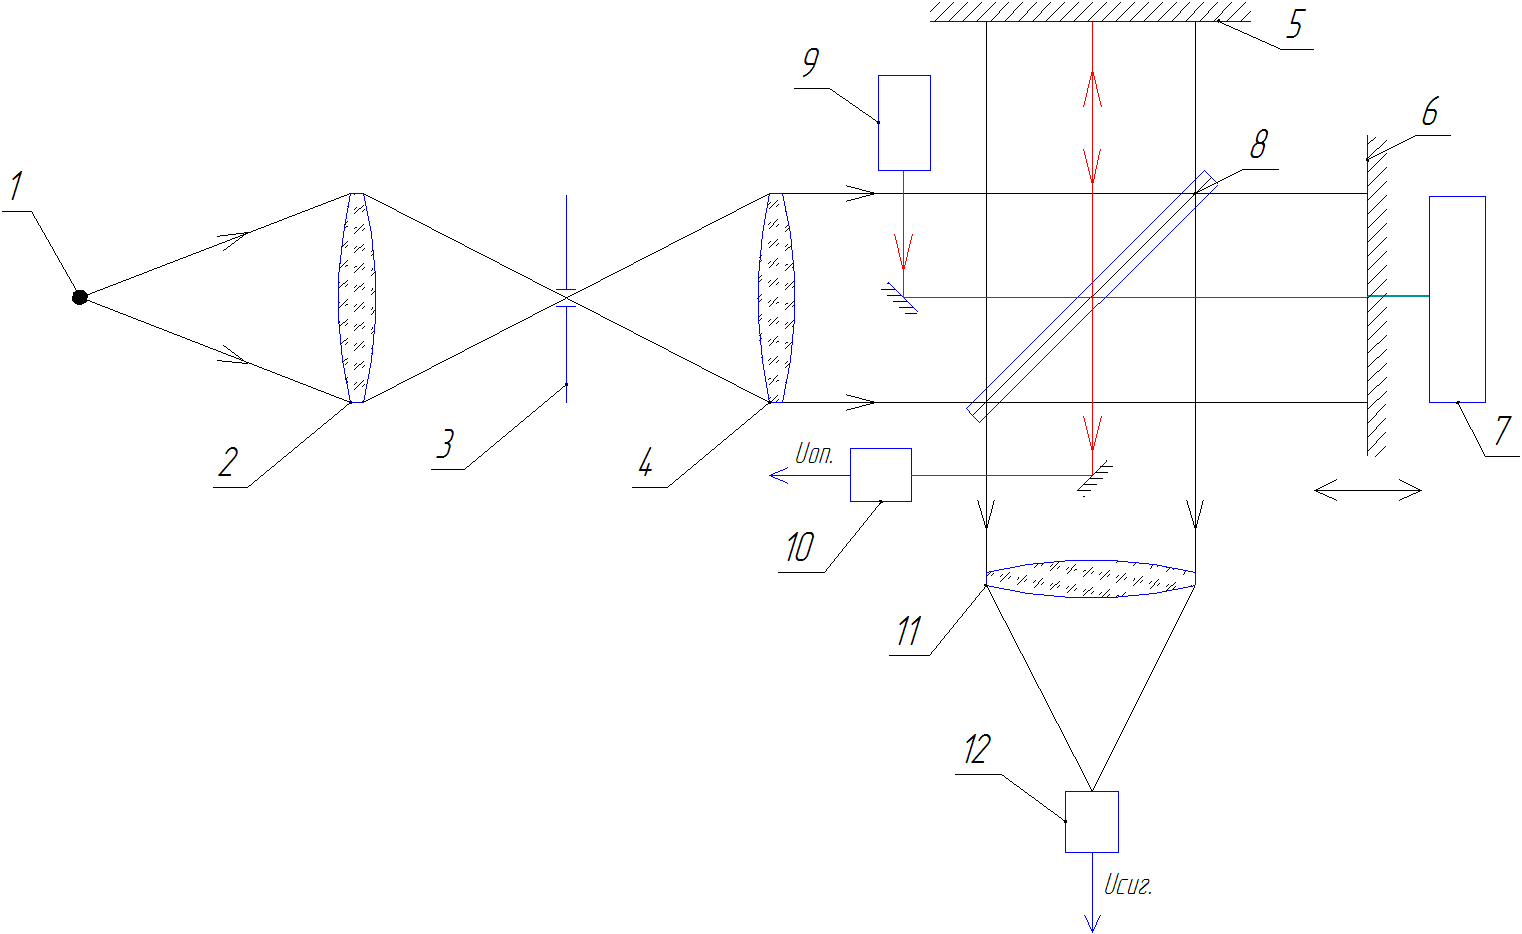
\includegraphics[width=0.5\textwidth]{1interf.png}
  \caption{Схема интерферометра Майкельсона}
  \end{figure}
	\item Схема Юнга -- как минимум, сильно ограниченная интерферограмма из-за огибающей от дифракции на одной щели.
	\item Интерферометры Релея и Жамена -- требуют точного измерения давления (и знания точной зависимости показателя преломления от давления), не позволяют удобно и быстро. менять разность хода, имеют собственный спектр поглощения
	\item Оптоволоконный интеферометр -- работает в узких спектральных диапазонах, требует дорогостоящего высокотехнологичного оборудования.
	\begin{figure}[H]
	\centering
  	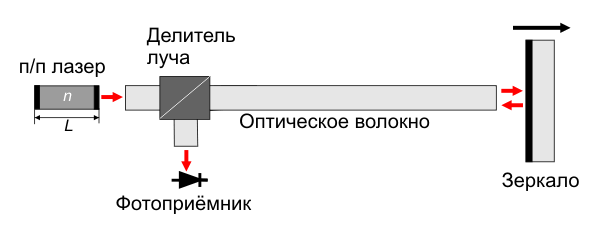
\includegraphics[width=0.5\textwidth]{4interf.png}
  \caption{Схема оптоволоконного интерферометра}
  \end{figure}
\end{enumerate}

\newpage
\section*{Интерференция на клине: спектр из ниоткуда}
	Окончательно было принято решения из всех интерференционных схем выбрать, быть может, не самую точную, но <<надежную>>, не зависящую ни от размера щелей, ни от радиуса пространственной когерентности схему.
	
	Удобной оказалась интерференция на двух плоскопараллельных пластинках, установленных под известным углом друг к другу (два покровных стекла, сжатых вместе и отделенных с одной стороны слоем известной толщины). Природа полос такая же, как в схеме колец Ньютона, однако полосы прямые и разность хода линейно зависит от смещения, что дает возможность получить достаточно длинную интерферограмму.
	
	\subsection*{Интерференционная картина}
	
	\begin{figure}[H]
		\centering
  		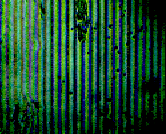
\includegraphics{waves.png}
  		\caption{Интерференционные полосы на пластинках}
	\end{figure}
	
	Интерференция наблюдается в отраженном свете, что создает существенную проблему: опеспечить минимальную засветку поля зрения, осветив при этом максимальную площадь поверхности. Несовершенство имеющегося оборудования и отсутствие достаточного количества времени сделали эту проблему критической, в результате был достигнут некий оптимальный результат, изображенный на рисунке.
	
	Очевидно, такой картины недостаточно для того, чтобы прописать содержательную интерферограмму, поэтому пришлось перемещать поверхность пластинок и делать последовательные фотографии, с тем, чтобы их впоследствии <<сшить>>. 
	
	В качестве источника света использовалась \textbf{ртутная лампа (ДРЛ)}, как источник с достаточно простым легко проверяемым спектром.

\newpage
	\subsection*{Обработка данных}
	
	\subsubsection*{Исходные изображения}
	В силу упомянутой проблемы малой освещенной области интерференционная картина занимала лишь малую часть матрицы зеркального фотоаппарата:
	\begin{figure}[H]
	\centering
  	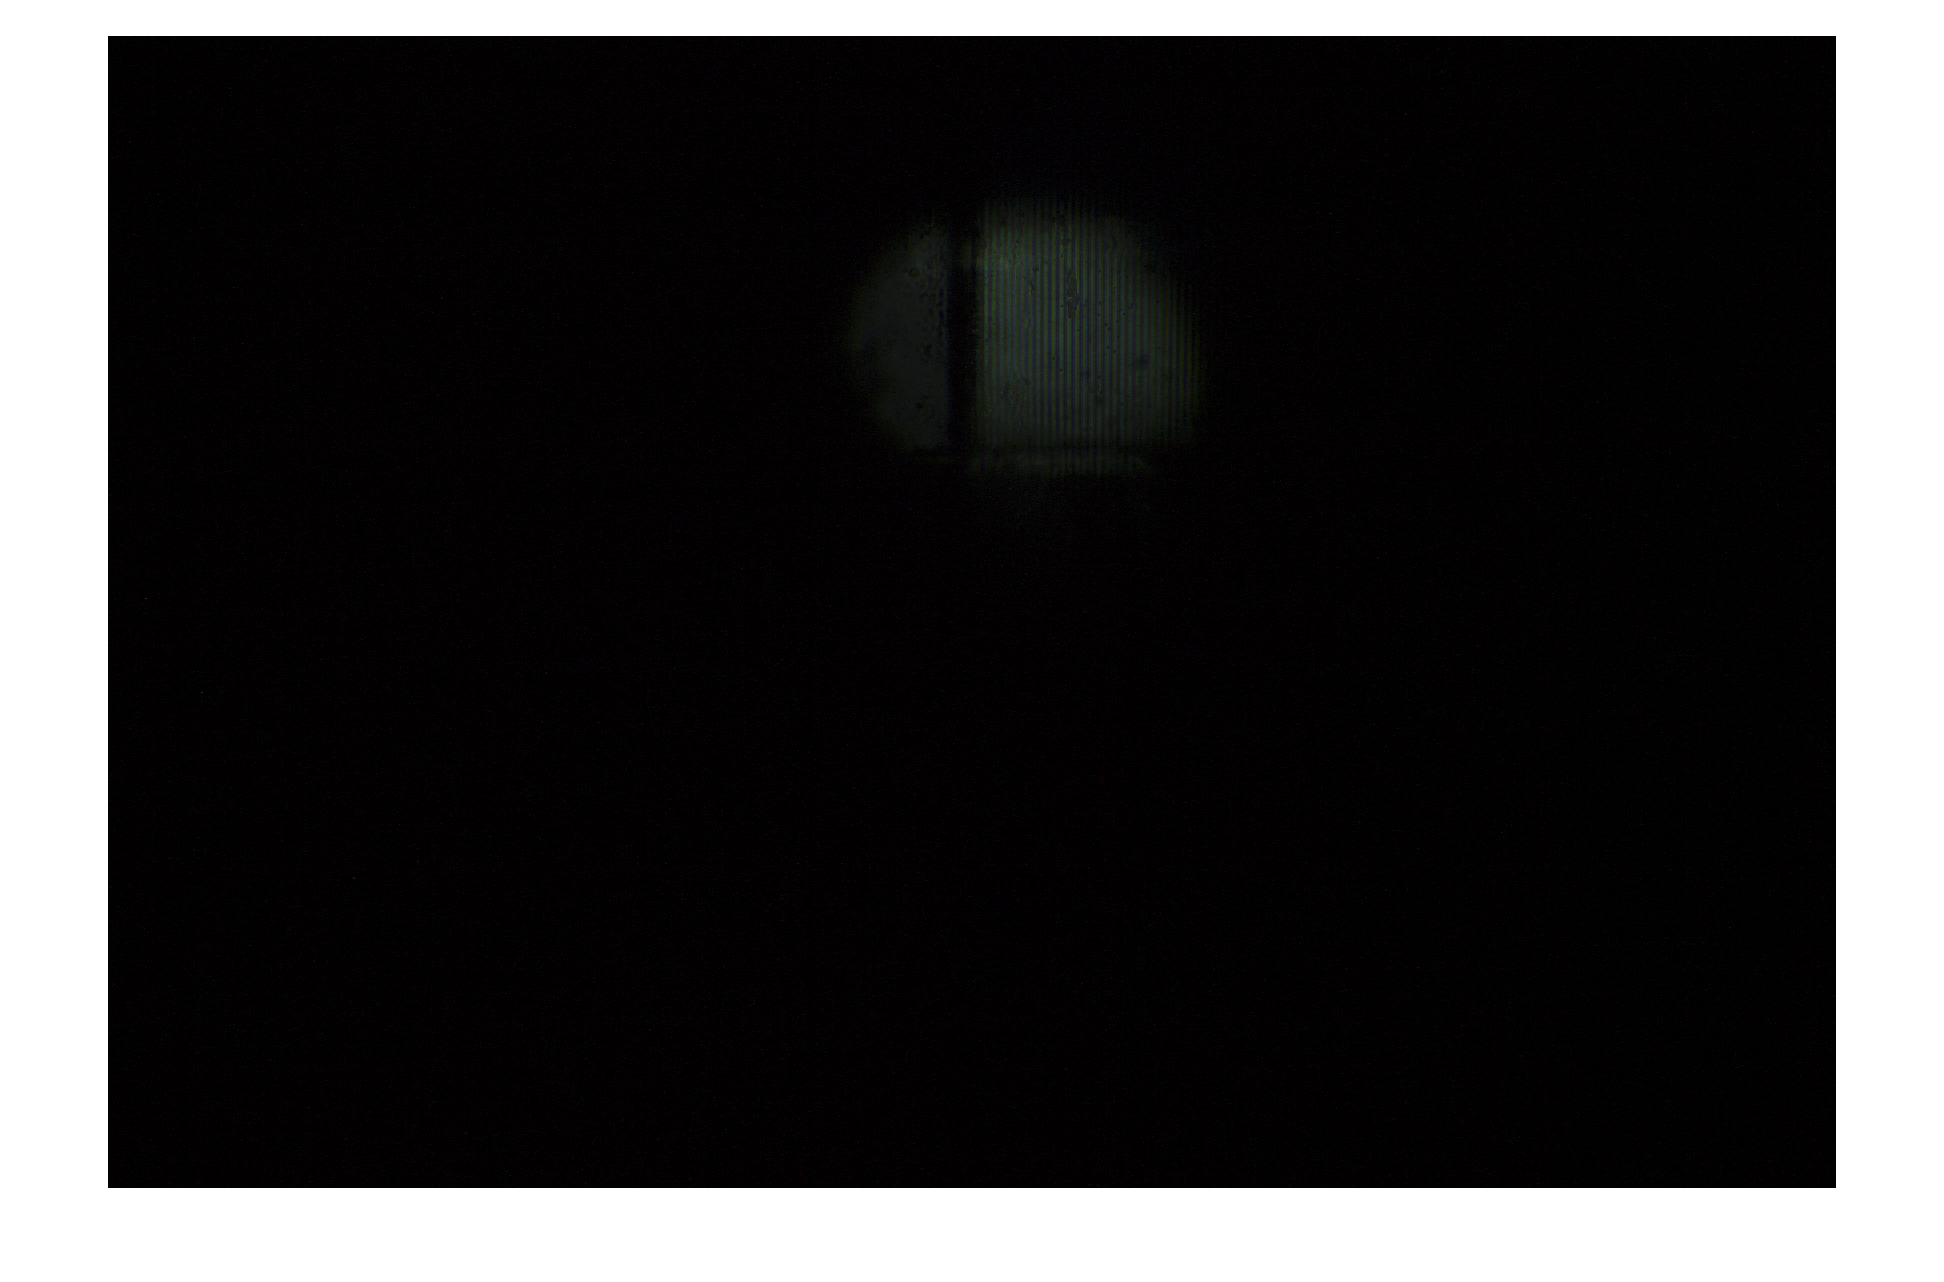
\includegraphics[width=0.7\textwidth]{waves_copy.png}
  \caption{Одна из исходных фотографий}
  \end{figure}
  
  50 отснятых фотографий подвергались пакетной обработке с помощью набора скриптов, написанных в среде \text{MATLAB}:
  \begin{enumerate}
  	\item Совмещение фотографий с помощью вычисления корелляции между последовательными фотографиями при различных смещениях
  	\begin{figure}[H]
	\centering
  	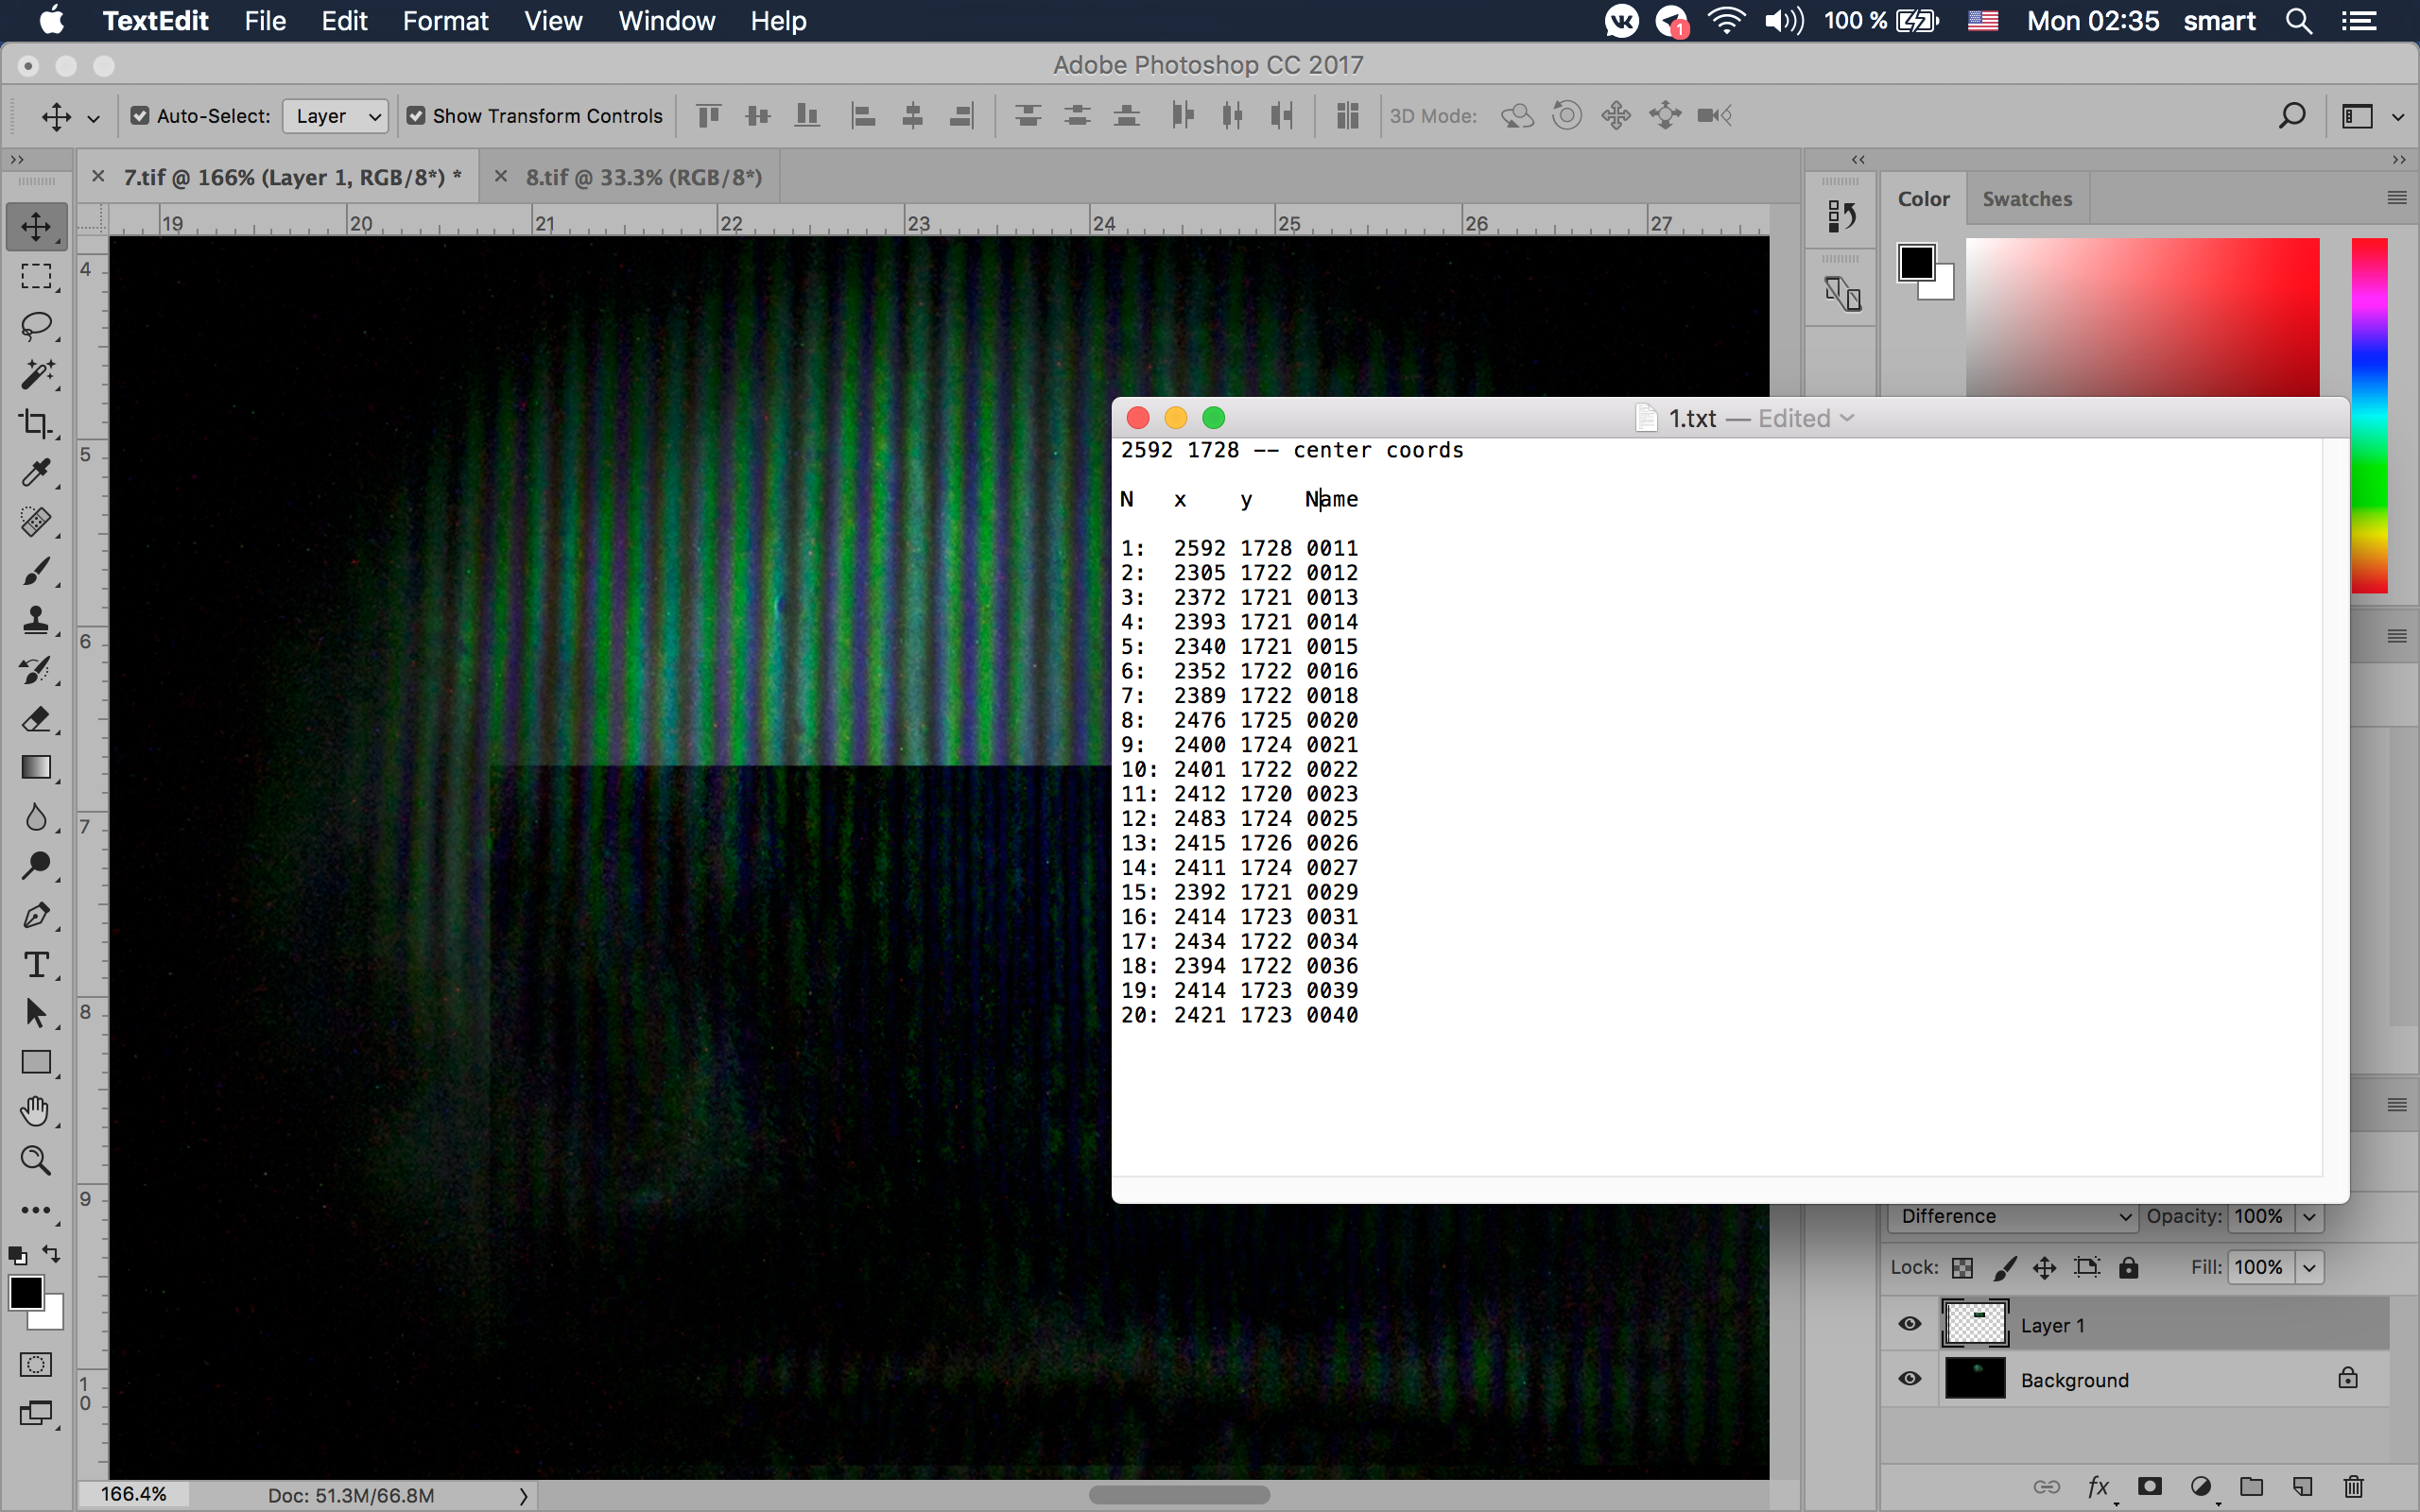
\includegraphics[width=0.7\textwidth]{ph.png}
  \caption{Совмещение фотографий <<вручную>> для проверки работы алгоритма}
  \end{figure}
  
  	\item Автоматическая обрезка фотографии с выбором наиболее релеватного участка (с наименьшей замусоренностью):
  	
  	\begin{figure}[H]
	\centering
  	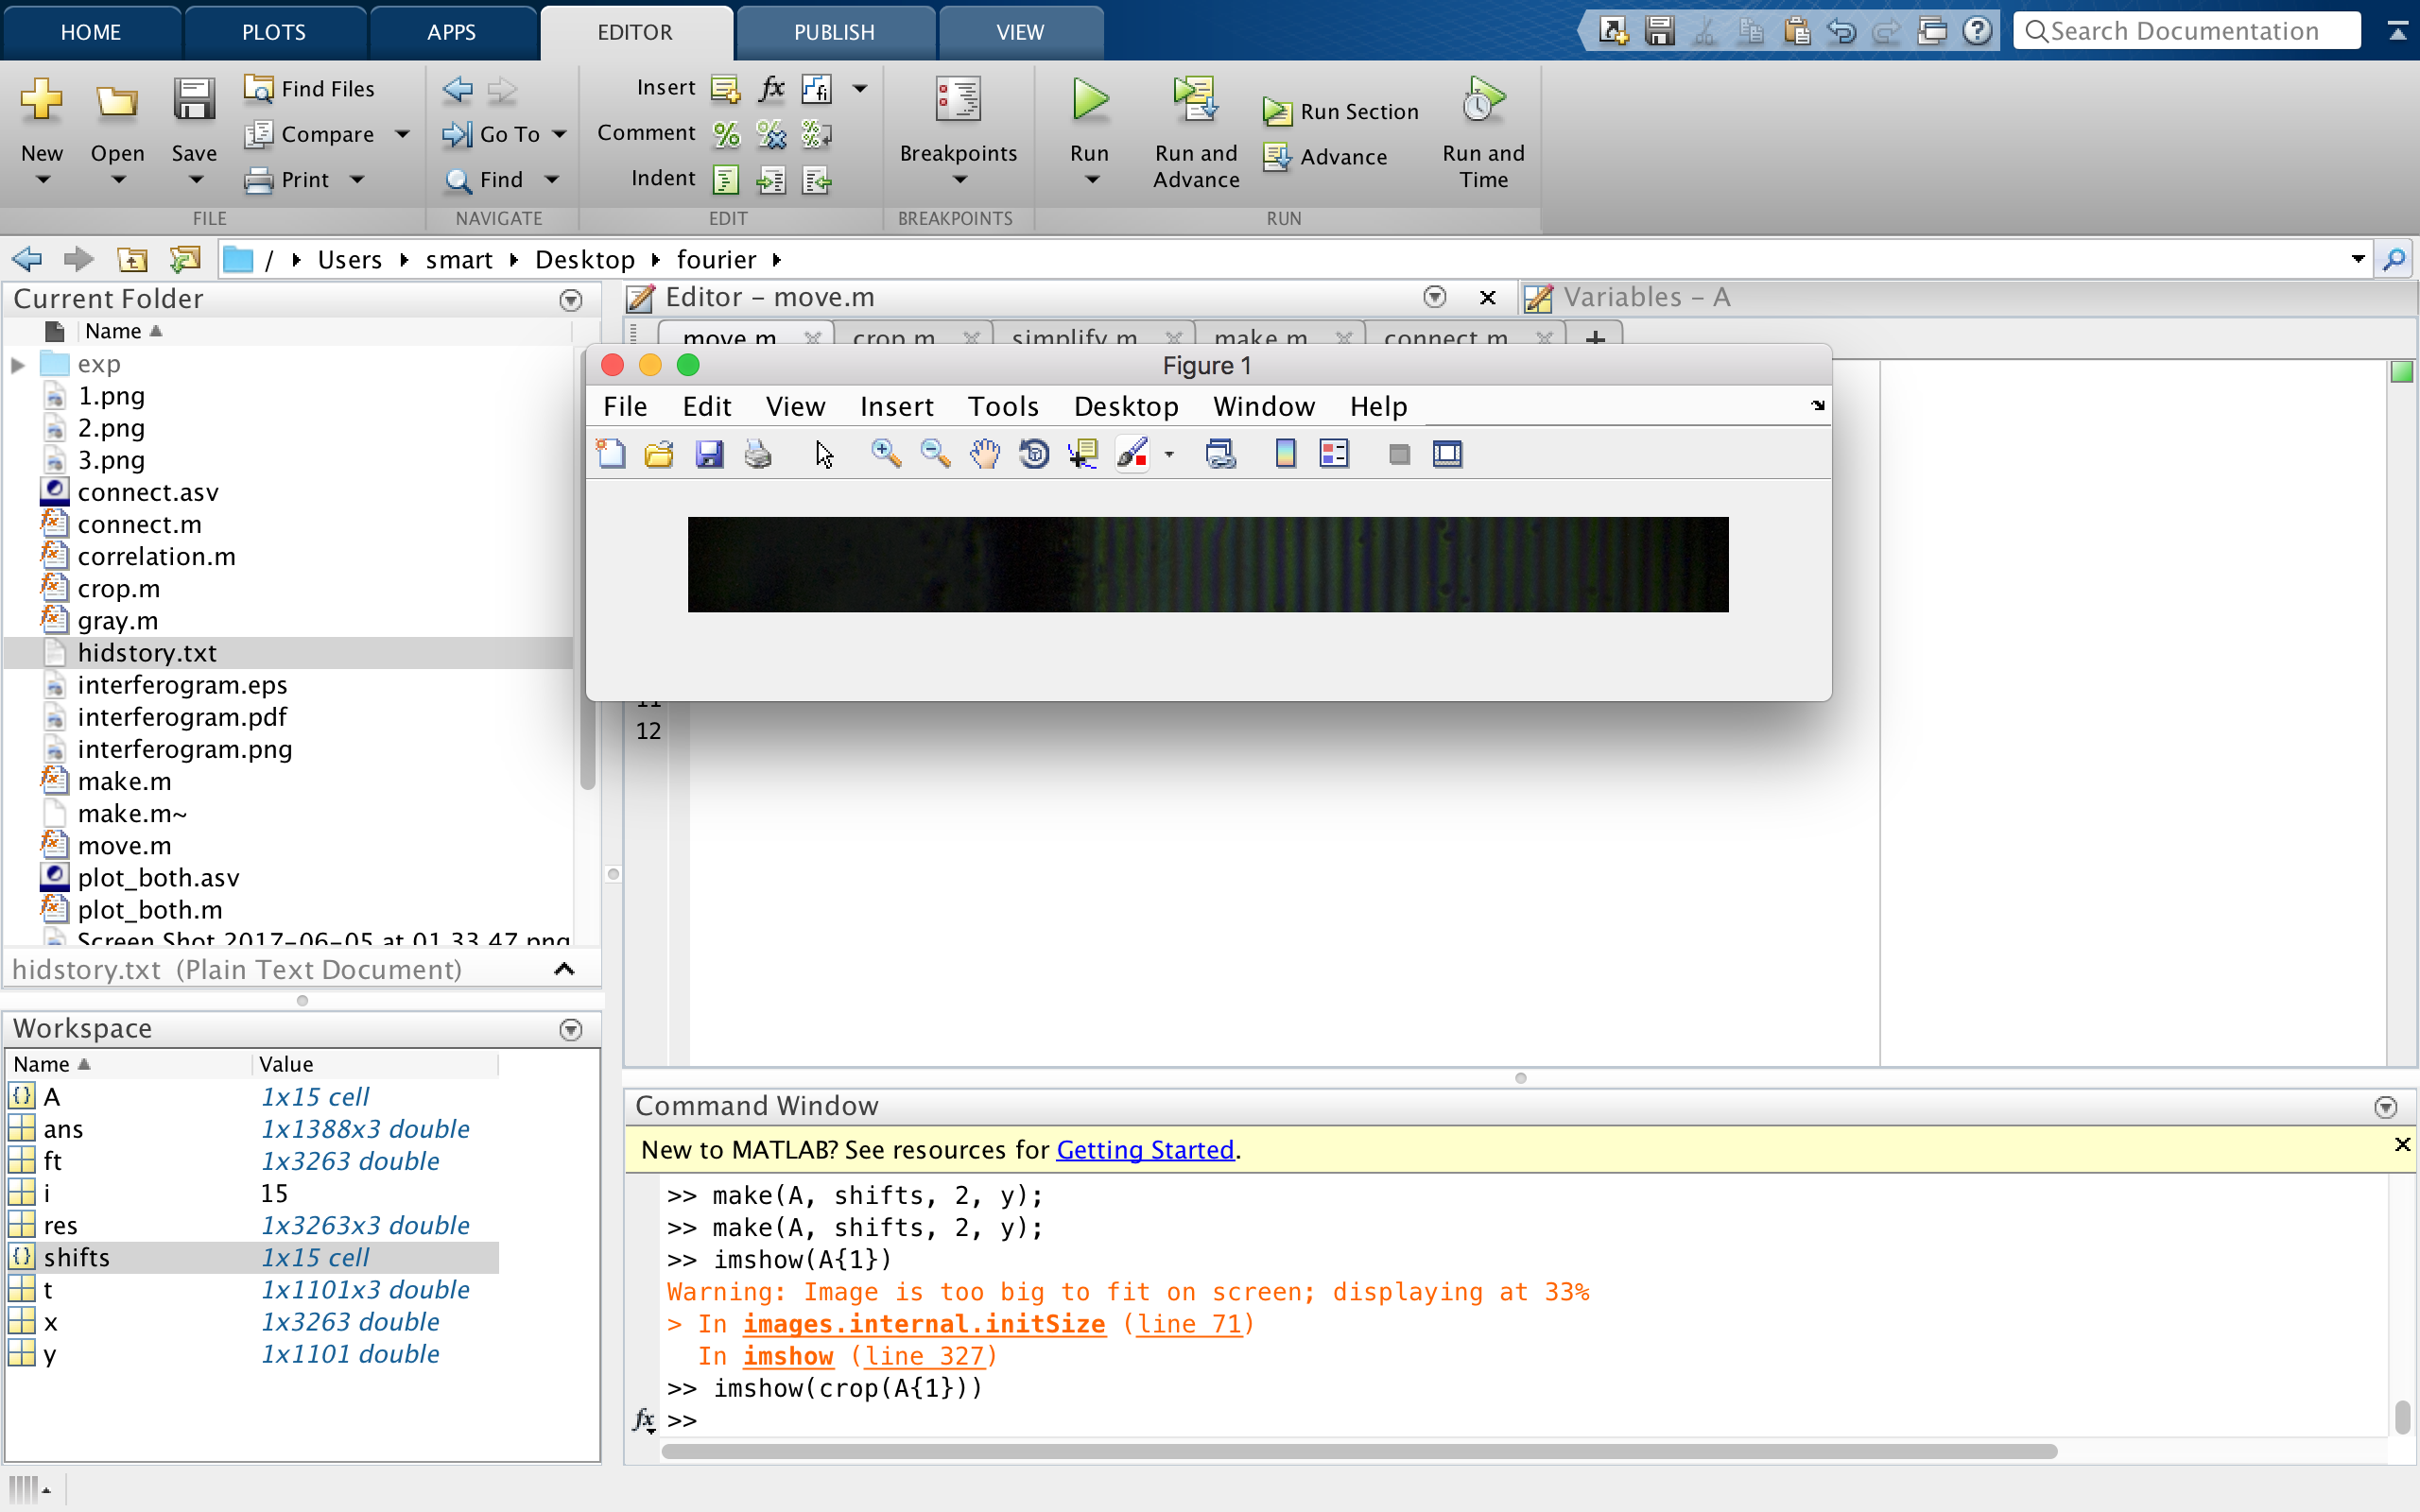
\includegraphics[width=0.7\textwidth]{crop.png}
  \caption{Обрезка скриптом в \text{MATLAB}}
  \end{figure}
  
  \item Построчное суммирование кадра и переход от фотографии к линейному массиву чисел (относительных единиц интенсивности каждого пикселя)
  \item Выравнивание средней интенсивности интерференционной картины вдоль кадра:
  \begin{figure}[H]
  \centering
  	\begin{minipage}[t]{0.7\textwidth}
  		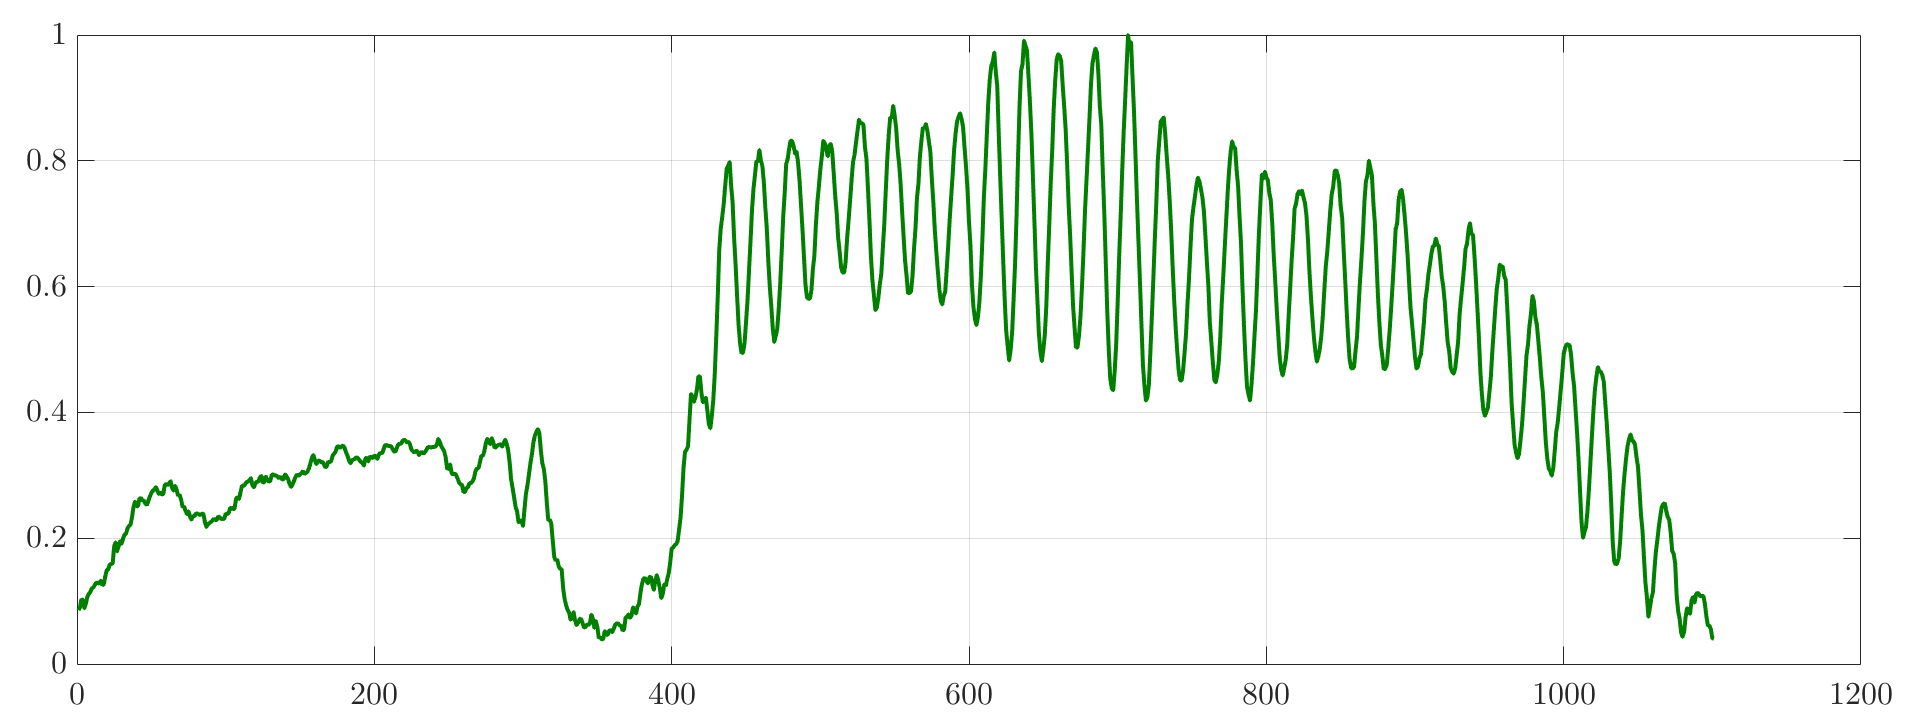
\includegraphics[width=\textwidth]{before.png}
  	\end{minipage}
  	\centering
  	\begin{minipage}[t]{0.7\textwidth}
  		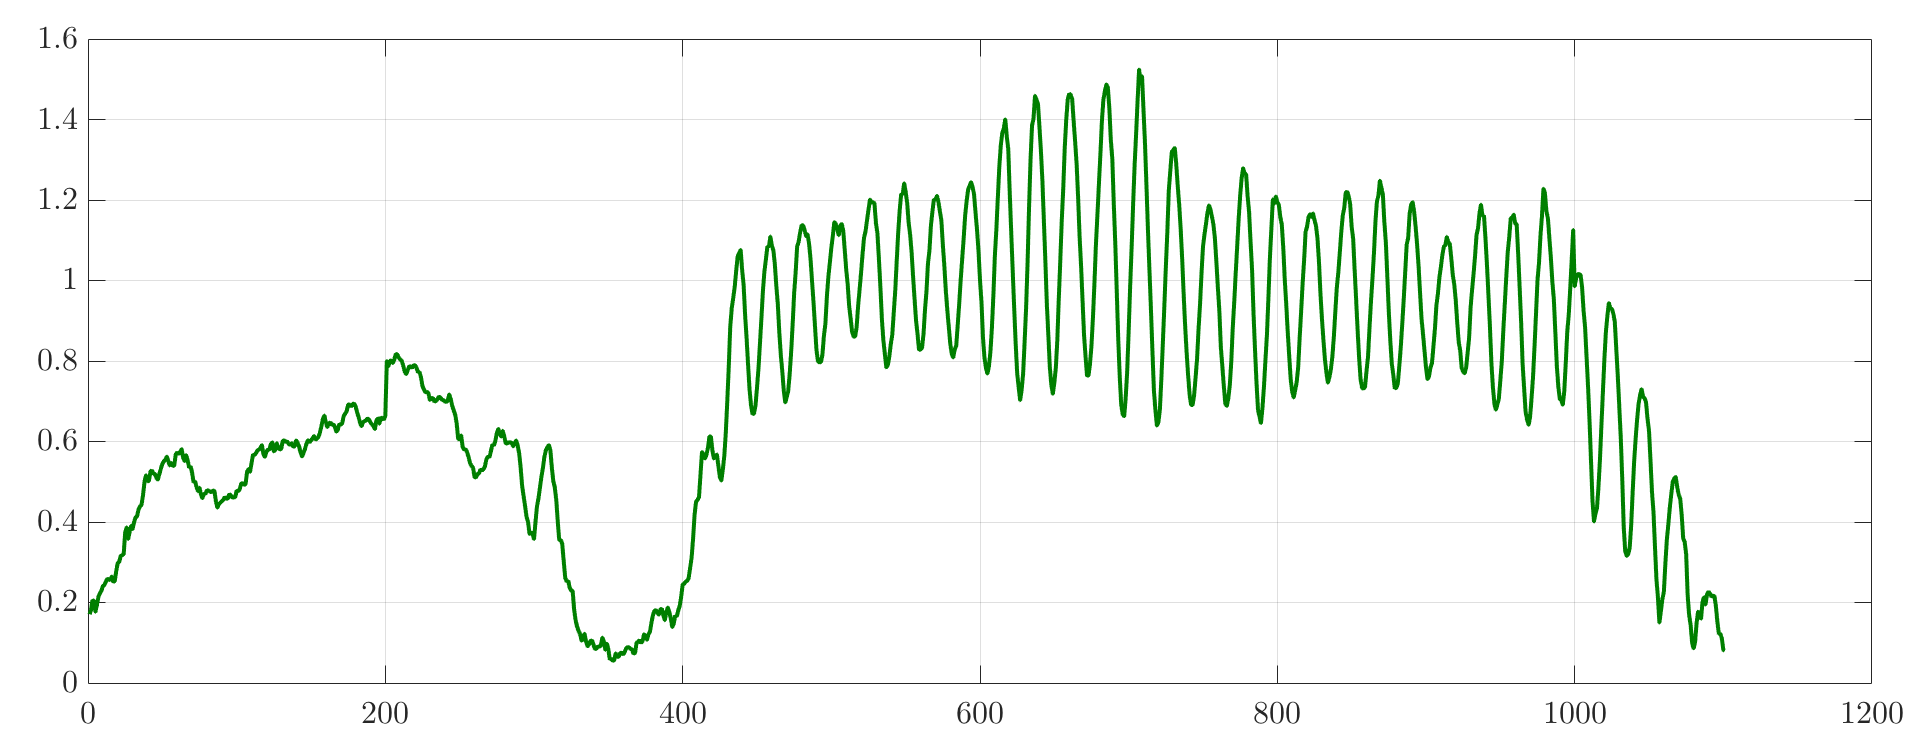
\includegraphics[width=\textwidth]{after.png}
  	\end{minipage}
  	\caption{До и после выравнивания интенсивности}
  \end{figure}
  
  \item Гладкая <<сшивка>> функций наложением огибающей, дающей среднее арифметическое в точке пересечения, также найденной алгоритмом:
  
  \begin{figure}[H]
  \centering
  	\begin{minipage}[t]{0.7\textwidth}
  		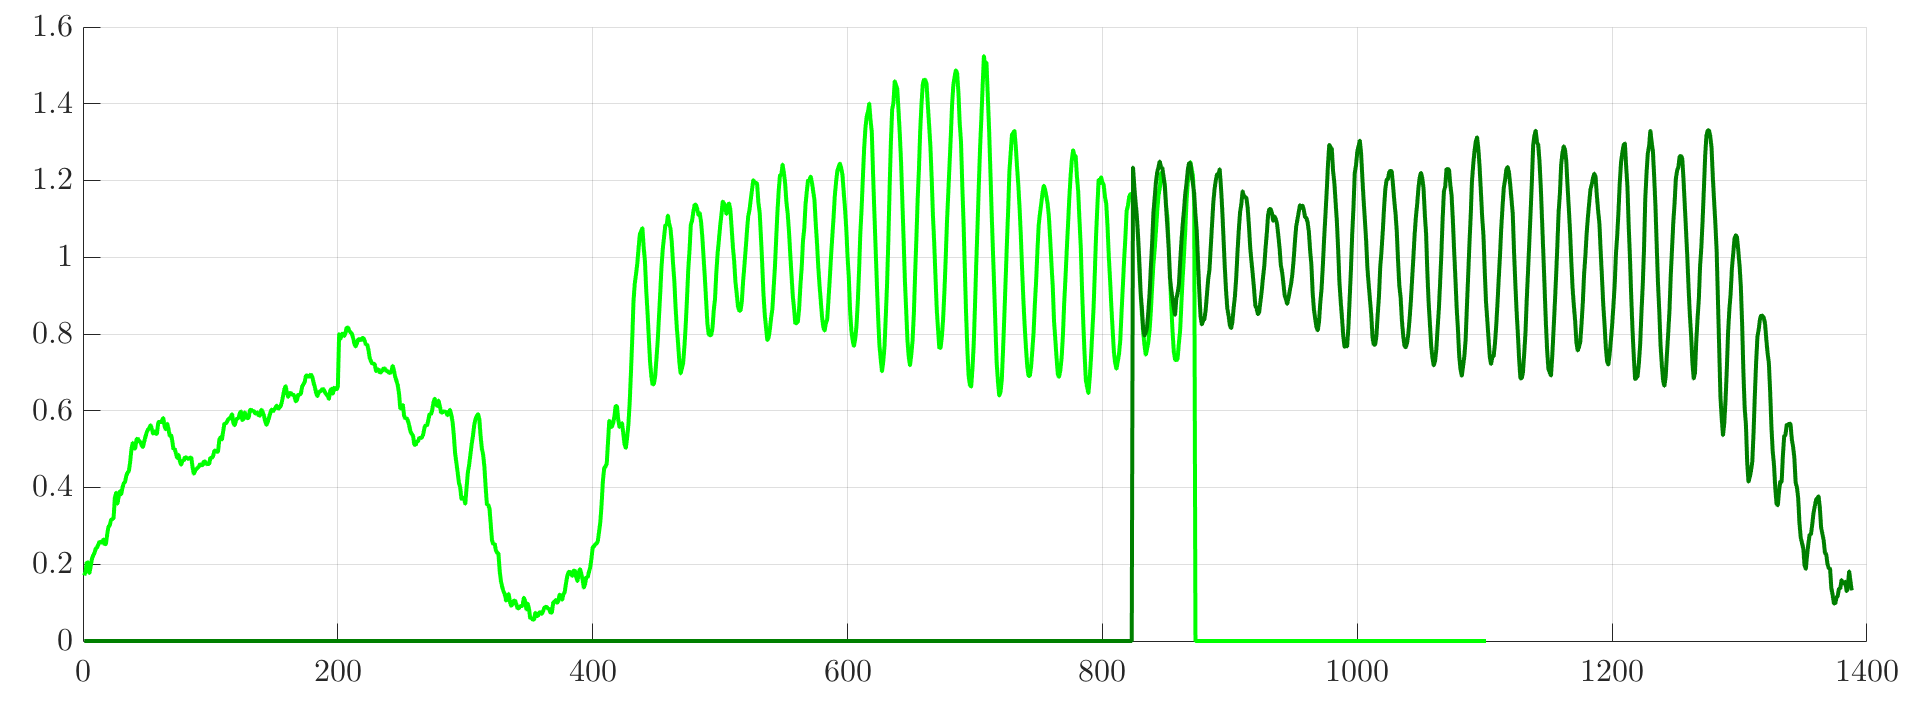
\includegraphics[width=\textwidth]{1.png}
  	\end{minipage}
  	\centering
  	\begin{minipage}[t]{0.7\textwidth}
  		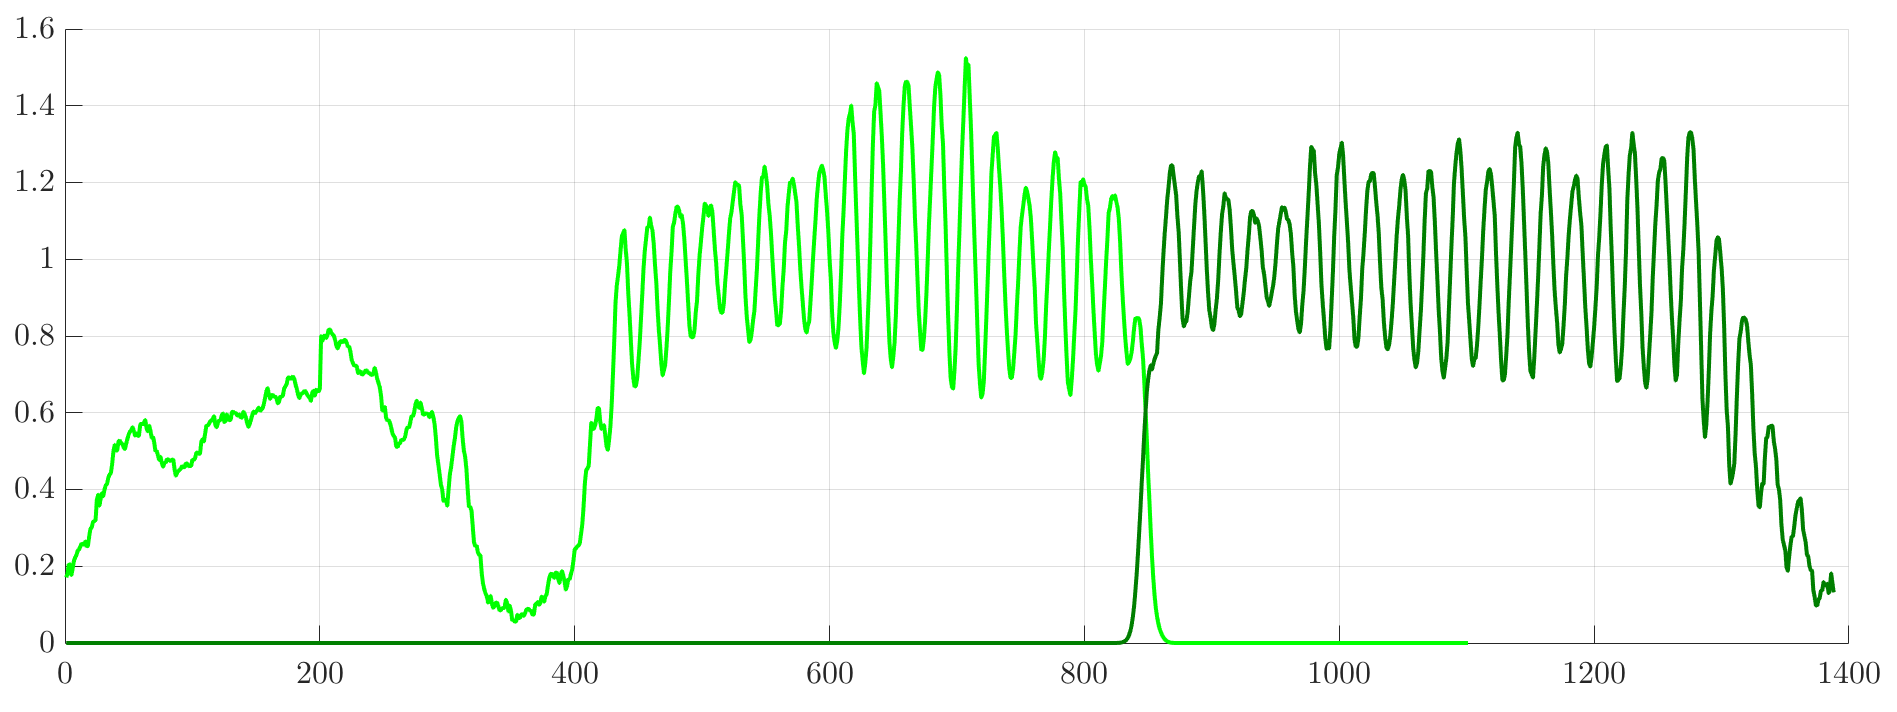
\includegraphics[width=\textwidth]{2.png}
  	\end{minipage}
  	\centering
  	\begin{minipage}[t]{0.7\textwidth}
  		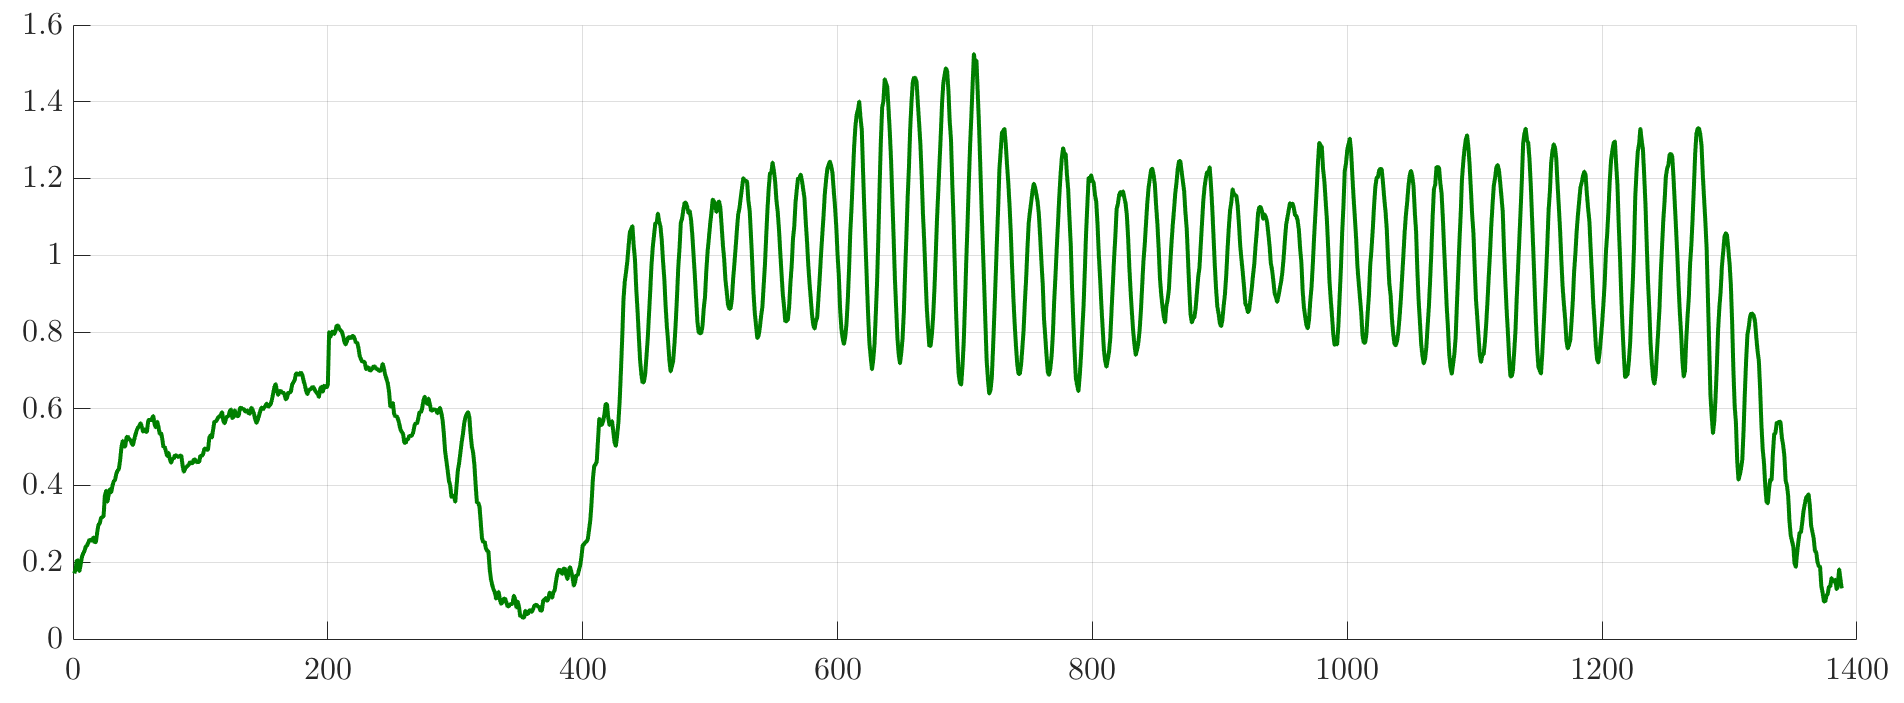
\includegraphics[width=\textwidth]{3.png}
  	\end{minipage}
  	\caption{Последовательные этапы <<сшивки>>}
  \end{figure}
  \end{enumerate}
  
  
	
	
	В итоге была получена достаточно длинная интерферограмма (\textbf{здесь и далее, если не указано иное, по оси абсцисс указано номер пикселя, по вертикали отложены относительные единицы, пропорциональные интенсивности}):
	\begin{figure}[H]
	\centering
  	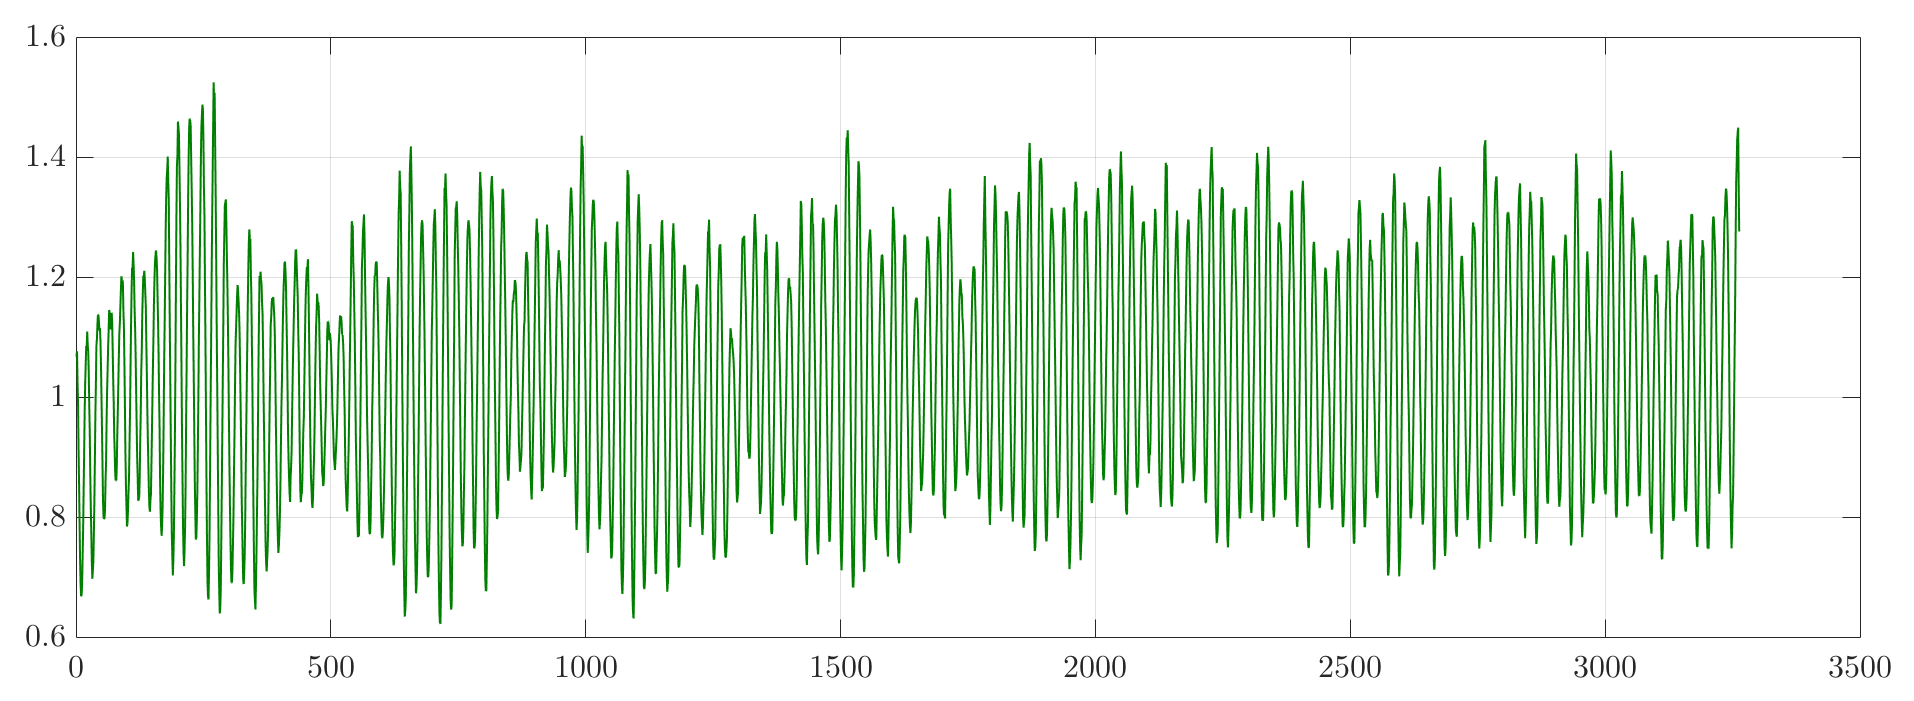
\includegraphics[width=\textwidth]{interferogram.png}
  \caption{Интерферограмма}
\end{figure}

\newpage
	\subsection*{Результаты и сравнение с известными параметрами спектра}
	
	Вычислив дискретное преобразование Фурье от полученной интерферограммы, получим спектр излучения ртутной лампы:
	
	\begin{figure}[H]
	\centering
  	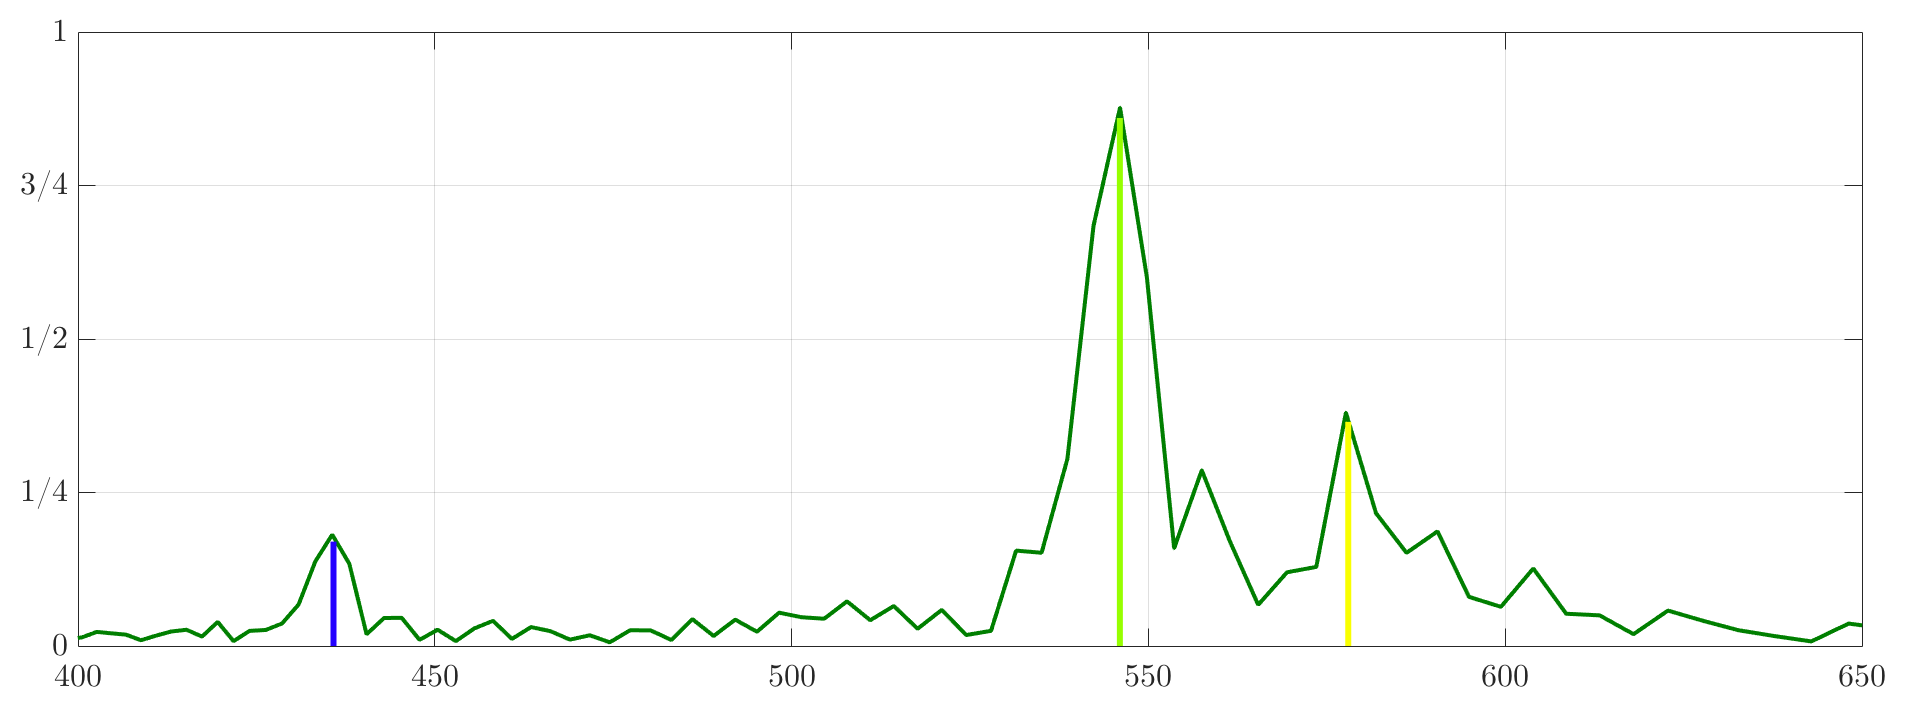
\includegraphics[width=\textwidth]{spectr.png}
  \caption{Спектр ртутной лампы, вычисленный по ДПФ интерферограммы}
  \end{figure}
  На графике цветными вертикальными линиями обозначены известные значения длин волн самых ярких линий ртутной лампы.
  
  Абсолютные значения совпали с точностью $\varepsilon = 0,1\%$.

	
\section*{Выводы}
\begin{enumerate}
	\item Изучен принцип Фурье-спектроскопии
	\item Исследованы перспективы использования различных интерференционных схем для реализации указанного метода
	\item Использована схема с двумя полоскопараллельными пластинками
	\item Получен спектр ртутной лампы, проверена адекватность и применимость Фурье-спектроскопии в реальных условиях
\end{enumerate}

\end{document}